%; whizzy paragraph -pdf xpdf -latex ./whizzypdfptex.sh
%; whizzy-paragraph "^\\\\begin{frame}\\|\\\\emtext"
% latex beamer presentation.
% platex, latex-beamer でコンパイルすることを想定。

%     Tokyo Debian Meeting resources
%     Copyright (C) 2012 Junichi Uekawa
%     Copyright (C) 2016 Nobuhiro Iwamatsu

%     This program is free software; you can redistribute it and/or modify
%     it under the terms of the GNU General Public License as published by
%     the Free Software Foundation; either version 2 of the License, or
%     (at your option) any later version.

%     This program is distributed in the hope that it will be useful,
%     but WITHOUT ANY WARRANTY; without even the implied warreanty of
%     MERCHANTABILITY or FITNESS FOR A PARTICULAR PURPOSE.  See the
%     GNU General Public License for more details.

%     You should have received a copy of the GNU General Public License
%     along with this program; if not, write to the Free Software
%     Foundation, Inc., 51 Franklin St, Fifth Floor, Boston, MA  02110-1301 USA

\documentclass[cjk,dvipdfmx,12pt]{beamer}
\usetheme{Tokyo}
\usepackage{monthlypresentation}

%  preview (shell-command (concat "evince " (replace-regexp-in-string "tex$" "pdf"(buffer-file-name)) "&")) 
%  presentation (shell-command (concat "xpdf -fullscreen " (replace-regexp-in-string "tex$" "pdf"(buffer-file-name)) "&"))
%  presentation (shell-command (concat "evince " (replace-regexp-in-string "tex$" "pdf"(buffer-file-name)) "&"))

%http://www.naney.org/diki/dk/hyperref.html
%日本語EUC系環境の時
\AtBeginDvi{\special{pdf:tounicode EUC-UCS2}}
%シフトJIS系環境の時
%\AtBeginDvi{\special{pdf:tounicode 90ms-RKSJ-UCS2}}

\newenvironment{commandlinesmall}%
{\VerbatimEnvironment
  \begin{Sbox}\begin{minipage}{1.0\hsize}\begin{fontsize}{8}{8} \begin{BVerbatim}}%
{\end{BVerbatim}\end{fontsize}\end{minipage}\end{Sbox}
  \setlength{\fboxsep}{8pt}
% start on a new paragraph

\vspace{6pt}% skip before
\fcolorbox{dancerdarkblue}{dancerlightblue}{\TheSbox}

\vspace{6pt}% skip after
}
%end of commandlinesmall

\newcommand{\textframe}[1]{
	\begin{frame}{}
	\begin{center}
	 {\Huge #1
		  }
	 \end{center}
	 \end{frame}
}


\title{Raspberry Pi3 / arm64}
\subtitle{Debian/Ubuntu ミートアップ in 札幌}
\author{岩松 信洋}
\date{2016年6月17日}
\logo{
\includegraphics[width=8cm]{image200607/openlogo-light.eps}}

\begin{document}

\begin{frame}
\titlepage{}
\end{frame}


\begin{frame}{自己紹介}

\begin{itemize}
\item 名前: 岩松 信洋(いわまつ のぶひろ) @iwamatsu
\item Debian Project Official Developer
\item Debian でのお仕事: Debian linux kernel, Debian Bluetooth, Debian Science (OpenCV), Erlang, Debian Go
\item 普段のお仕事: Linux kernel 開発、U-Boot メンテナ、Yocto Project
\end{itemize} 
\end{frame}

%\begin{frame}{Agenda}
%  \begin{itemize}
%   \item Debian とは?
%   \item Debian Updates
%   \item 今後のイベント
%  \end{itemize}
%\end{frame}
%
%\section{Debian とは?}
%\begin{frame}\begin{center}\Huge{Debian とは?}\end{center}\end{frame}

\begin{frame}{Raspberry Pi 3/RPi3}

\begin{itemize}
\item 2016/2/29 販売開始
\item Broadcom BCM2837 Cortex-A53 1.2Ghz Quad-core
\item aarch64 (ARM 64bit)
\item メモリ 1GB
\item WiFiとBluetooth 搭載
\end{itemize}

\begin{center}
%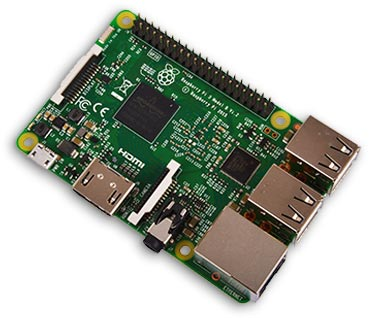
\includegraphics[width=0.5\hsize]{image201606/3141592653.jpg}
\end{center}
{\tiny \url{http://uk.rs-online.com/web/generalDisplay.html?id=raspberrypi}より。}

\end{frame}

\begin{frame}{Raspberry Pi 3/RPi3}

\begin{itemize}
\item デフォルト サポートOS
\begin{itemize}[<+->]
	\item Raspbian
	\item \color{red}{armhf (浮動小数点演算ハードウェアサポート)}
	\item \color{red}{32bitバイナリ。64bit ではない}
\end{itemize}
\end{itemize}

\end{frame}

\begin{frame}{Raspberry Pi 3/RPi3}

\begin{itemize}
\item ハードウェアが64bitなのにソフトウェアは32bitのみサポート
\item 64bit の恩恵を受けたい。

\begin{itemize}
	\item 国内で容易に購入できる貴重なaarch64デバイス
	\item レジスタサイズ、アドレス空間
	\item etc
\end{itemize}
\item インターネット上で有志による移植が開始される。
\end{itemize}

\end{frame}

\begin{frame}{RPi3 Linux arm64化までの歴史}

\begin{enumerate}[<+->]
\item RPi3 販売当初は32bit のみ対応 \\
   stub (デバイス初期プログラム) が 32bit サポートのみ。\\
   Linuxカーネルも未対応。\\
   早速Rpi のフォーラムで64bit化の話題が作成される。\\
   \ \ {\tiny \url{https://www.raspberrypi.org/forums/viewtopic.php?f=66&t=138385}}

\item 2016/3/26 にGithub にバグレポートされる。\\
   \ \ {\tiny \url{https://github.com/raspberrypi/firmware/issues/579}}
\end{enumerate}
\end{frame}

\begin{frame}{RPi3 Linux arm64化までの歴史}
\begin{enumerate}
\setcounter{enumi}{3}
\item Stephen Warren 氏(U-Boot / Nvidia / Rpi メンテナ) によって stub が開発される。
   \ \ {\tiny \url{https://github.com/swarren/rpi-3-aarch64-demo}}

\item Raspberry Pi Foundation が 64bit(armv8) 向けstubを公開。 \\
   \ \ {\tiny \url{https://github.com/raspberrypi/tools.git}}

\end{enumerate}
\end{frame}

\textframe{RPi3 Linux arm64 サポート状況}

\begin{frame}[containsverbatim]{クロスコンパイラ}

Debian stretch/sid では 公式リポジトリからインストール可能。Ubuntuも同様に可能。

\begin{commandline}
$ sudo apt install gcc-aarch64-linux-gnu
\end{commandline}
%$

\end{frame}

\begin{frame}{ブートローダ}

\begin{itemize}
\item 基本ブートローダ不要なデバイスだが、RPi3/aarch64 Linuxカーネルが開発途中のため
いろいろいじれるようにするためにネットワーク/USBブートができるよう環境を整え
ておいたほうが楽。
\item 組込機器でよく利用されるU-Bootをでは既にサポートされているため、SDカードに組み込んで
置く。
	{\small \url{git://git.denx.de/u-boot.git}}
\end{itemize}

\begin{center}
\includegraphics[width=0.8\hsize]{image201606/boot.eps}
\end{center}

\end{frame}

\begin{frame}{Linux カーネル}

\begin{itemize}
  \item LKMLにはサポート用パッチが投稿されている。4.8、4.9 にはサポートが入る動き。
  \begin{center}
  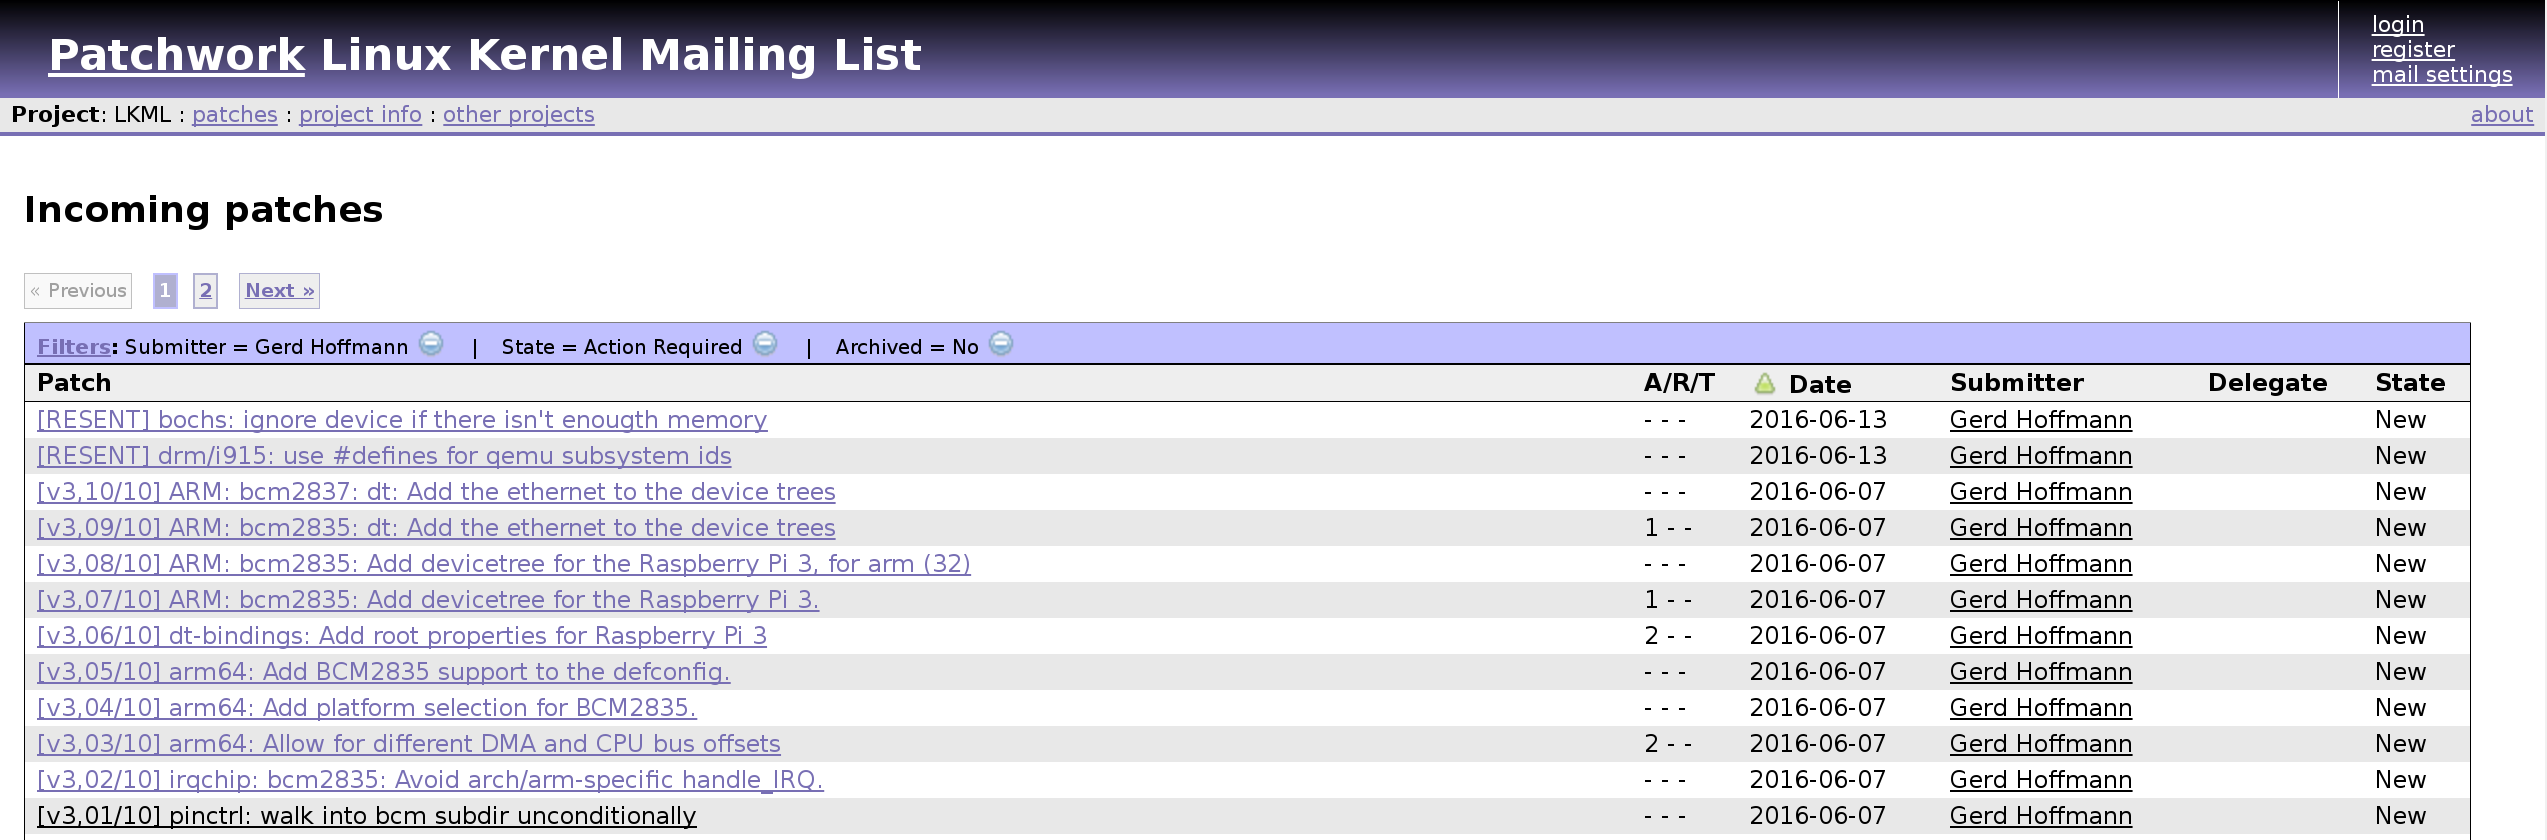
\includegraphics[width=0.8\hsize]{image201606/patchwork.png}
  \end{center}
  \item Raspberry Pi Foundation ではまだ未サポート。 \\
   \ \ {\small \url{https://github.com/raspberrypi/linux/issues/1310}}
  \item 有志によって公開されているLinuxカーネルがいくつか存在。\\
    \ \ {\small \url{https://github.com/anholt/linux.git}} \\
    \ \ {\small \url{https://github.com/zeldin/linux.git}} \\
\end{itemize}

\end{frame}

\begin{frame}{ユーザランド}

\begin{itemize}
  \item Debian / Ubuntu で aarch64向けバイナリが提供。
  \item RedHat, Suse、Gentoo、Archなどの主要ディストリでもサポート。
\end{itemize}

\end{frame}

\textframe{RPi3 Debian/arm64 化方法}

\begin{frame}{arm64化の流れ}

\begin{enumerate}
  \item クロスコンパイラのインストール
  \item microSDカードのフォーマット・パーティション作成
  \item RPi3 ブートファイルの取得と/bootへのコピー
  \item U-Bootのソースコード取得とコンパイル
  \item Linux カーネルソースコードのコンパイル
  \item cdebootstrap を使ったmicroSDカードへのユーザランドインストール
\end{enumerate}

\end{frame}

\textframe{1. クロスコンパイラのインストール}

\begin{frame}[containsverbatim]{クロスコンパイラのインストール}
  \begin{commandline}
  $ sudo apt update
  $ sudo apt install gcc-aarch64-linux-gnu
  \end{commandline}
\end{frame}

\textframe{2. microSDカードのフォーマット・パーティション作成}

\begin{frame}[containsverbatim]{microSDカードの認識確認}

\begin{commandline}
$ dmesg  | tail -5
[869873.800361] sd 6:0:0:3: [sde] 15523840 512-byte logical blocks: (7.94 GB/7.40 GiB)
[869873.831121]  sde: sde1
\end{commandline}

\end{frame}

\begin{frame}[containsverbatim]{パーティションテーブル領域を初期化}

\begin{commandline}
$ sudo dd if=/dev/zero of=/dev/sde bs=1M count=1
\end{commandline}
%$

\end{frame}

\begin{frame}[containsverbatim]{microSDカードにパーティション作成/1}

第1パーティションは 32MB/FVAT ファイルシステム、
第2パーティションは残りサイズ/EXT4 ファイルシステムとして作成。

\begin{commandline}
$ sudo fdisk /dev/sde
Command (m for help): o
...
Command (m for help): n
...
Select (default p): p
...
Partition number (1-4, default 1): 1
...
Last sector, +sectors or +size{K,M,G,T,P} \
	     (2048-15523839, default 15523839): +32M
...
\end{commandline}
%$

\end{frame}

\begin{frame}[containsverbatim]{microSDカードにパーティション作成/2}

\begin{commandline}
Command (m for help): t
...
Hex code (type L to list all codes): e
...
Command (m for help): n
...
Select (default p): p
...
Partition number (2-4, default 2): 2
...
Command (m for help): w
\end{commandline}

\end{frame}

\begin{frame}[containsverbatim]{microSDカードにパーティション作成 ワンライナー版}
\begin{commandline}
(echo o; echo n; echo p; echo 1; echo ; echo +32M; \
 echo t; echo e; echo n; echo p; echo 2; echo ; echo ; \
 echo w) | fdisk /dev/sde
\end{commandline}
\end{frame}

\begin{frame}[containsverbatim]{microSDカードのフォーマット}
\begin{commandline}
$ sudo mkfs.msdos /dev/sde1
$ sudo mkfs.ext4 /dev/sde2
$ mkdir /tmp/boot /tmp/rootfs
$ sudo mount /dev/sde1 /tmp/boot
$ sudo mount /dev/sde2 /tmp/rootfs
\end{commandline}
\end{frame}

\textframe{3. RPi3 ブートファイルの取得と/bootへのコピー}

\begin{frame}[containsverbatim]{RPi3 ブートファイルの取得と/bootへのコピー}

  \begin{commandline}
  $ git clone --depth 1 \ 
  	https://github.com/raspberrypi/tools.git
  $ sudo cp -rf tools/boot/* /tmp/boot/
  \end{commandline}
\end{frame}

\textframe{4. U-Bootのソースコード取得とコンパイル}

\begin{frame}[containsverbatim]{U-Bootのソースコード取得とコンパイル}
  \begin{commandline}
  $ git clone git://git.denx.de/u-boot.git
  $ cd u-boot
  $ make rpi_3_defconfig
  $ make CROSS_COMPILE=aarch64-linux-gnu-
  $ sudo cp u-boot.bin /tmp/boot/
  $ cd ..
  \end{commandline}
\end{frame}

\begin{frame}[containsverbatim]{U-Boot用スクリプトの作成とコピー}
\begin{commandline}
$ cat << EOF > boot.scr
fatload mmc 0:1 \${fdt_addr_r} \${fdtfile}
fatload mmc 0:1 \${kernel_addr_r} image
setenv bootargs console=ttyS0,115200 \
	root=/dev/mmcblk0p2 rootfstype=ext4 rootwait rw
booti \${kernel_addr_r} - \${fdt_addr_r}
EOF
$ mkimage -A arm -O linux -T script -C none -a 0 \
	-e 0 -n "For Rpi3" -d boot.scr boot.scr.uimg
$ sudo cp boot.scr.uimg /tmp/boot/
\end{commandline}
\end{frame}

\begin{frame}[containsverbatim]{RPi3 ブート方法設定(config.txt)}
\begin{commandline}
$ cat << EOF | sudo tee /tmp/boot/config.txt > /dev/null
enable_uart=1
arm_control=0x200
kernel=u-boot.bin
hdmi_group=2
hdmi_mode=82
EOF
\end{commandline}
\end{frame}

\textframe{5. Linux カーネルのソースコード取得とコンパイル}

\begin{frame}[containsverbatim]{Linux カーネルのソースコード取得とコンパイル}
\begin{commandline}
$ git clone https://github.com/anholt/linux.git
$ cd linux
$ git checkout -b rpi3-devel origin/bcm2837-64-next
$ make ARCH=arm64 CROSS_COMPILE=aarch64-linux-gnu-
$ sudo cp arch/arm64/boot/Image /tmp/boot/
$ sudo cp arch/arm64/boot/dts/broadcom/bcm2837-rpi-3-b.dtb \
	/tmp/boot/
\end{commandline}
\end{frame}

\textframe{6. cdebootstrap を使ったmicroSDカードへのインストール}
\begin{frame}[containsverbatim]{cdebootstrap を使ったmicroSDカードへのインストール}

\begin{commandline}
$ sudo cdebootstrap --arch=arm64 -f standard \
  --foreign jessie \
  --include=openssh-server,ntp,ca-certificates,vim \
  /tmp/rootfs
...
\end{commandline}

\end{frame}

\begin{frame}[containsverbatim]{fstabの設定}

\begin{commandline}
$ cat << EOF | \
	sudo tee /tmp/rootfs/etc/fstab > /dev/null
proc            /proc  proc defaults	     0 0
/dev/mmcblk0p1  /boot  vfat defaults	     0 2
/dev/mmcblk0p2  /      ext4 defaults,noatime 0 1
EOF
\end{commandline}
%$

\end{frame}

\begin{frame}[containsverbatim]{ネットワークデバイスの設定}

\begin{commandline}
$ cat << EOF | \
	sudo tee /tmp/rootfs/etc/network/interfaces > \
	/dev/null
auto eth0
iface eth0 inet dhcp
\end{commandline}
%$

\end{frame}

\begin{frame}[containsverbatim]{rootfs用パーティションの変更}

\texttt{/tmp/rootfs/sbin/init} を編集。
\begin{commandline}
trap 'error "Interruped!"' HUP INT TERM

mount -n -o remount,rw rootfs / <- これを
mount -n -o remount,rw /dev/mmcblk0p2 / <- これに変更

chown -hR 0:0 /
\end{commandline}
\end{frame}

\begin{frame}[containsverbatim]{root のパスワードの設定とrpiユーザの追加}
\begin{commandline}
echo 'deb http://ftp.debian.org/debian jessie main' > \
	     /etc/apt/sources.list

echo "root:root" | chpasswd <- この行を追加
useradd -m rpi <- この行を追加
echo rpi:rpi | chpasswd <- この行を追加

run rm /sbin/init
\end{commandline}
\end{frame}

\begin{frame}[containsverbatim]{microSDカードのアンマウントとRPi2の起動}

\begin{enumerate}
\item microSDカードをアンマウントし、Ppi3 の microSDカードスロットに挿入する。
\item 挿入後、micro USB ケーブルを Rpi3 に挿し、Rpi3を起動する。
\item 起動すると自動的に2nd bootstrapが実行され、Rpi3上でインストールが実行される
\item 30分ほど待つ
\item インストール完了
\end{enumerate}
microSDカードへの詳細インストール方法は 2015年3月の勉強会資料
「Rapberry Pi 2 Model B に Debian Jessie / armhf をインストールする」
を参考。
\end{frame}

\textframe{ベンチマーク}
\begin{frame}[containsverbatim]{ベンチマーク}
Himeno Bench で測定
\begin{itemize}
	\item armhf (32bit)
		\begin{itemize}
			\item 1コア時: 79 MFLOPS
			\item 4コア時: 312 MFLOPS
		\end{itemize}
	\item aarch64 (64bit)
		\begin{itemize}
			\item 1コア時: 88 MFLOPS
			\item 4コア時: 334 MFLOPS
		\end{itemize}
\end{itemize}

1割ほど速い。

\end{frame}
%
\textframe{まとめ}
\begin{frame}[containsverbatim]{まとめ}

\begin{itemize}
\item Rapberry Pi 本家ではまだarm64は未サポートだが、有志によって環境が整っている。
\item Linux Vanilla カーネルの方にパッチが投稿されている。Linuxでの正式サポートも時間の
問題と思われる。
\item Himeno Benchの結果を見る限り、armhf より1割ほど速い。
\item グラフィックなどの対応はまだ未調査。
\item arm64環境でカーネルなどの低レイヤーでいろいろ遊びたい人には移行するよいタイミング。
\end{itemize}
\end{frame}

\end{document}

;;; Local Variables: ***
;;; outline-regexp: "\\([ 	]*\\\\\\(documentstyle\\|documentclass\\|emtext\\|section\\|begin{frame}\\)\\*?[ 	]*[[{]\\|[]+\\)" ***
;;; End: ***
